              
% --------------------------------------------------------------
% This is all preamble stuff that you don't have to worry about.
% Head down to where it says "Start here"
% --------------------------------------------------------------
 
\documentclass[11pt]{article}
\usepackage[utf8]{inputenc} 
\usepackage[margin=1in]{geometry}
\usepackage{graphicx}
\usepackage{float}
\usepackage{hyperref} 
\usepackage{amsmath,amsthm,amssymb}
\usepackage[table]{xcolor}
 
\newcommand{\N}{\mathbb{N}}
\newcommand{\Z}{\mathbb{Z}}
 
\newenvironment{theorem}[2][Theorem]{\begin{trivlist}
\item[\hskip \labelsep {\bfseries #1}\hskip \labelsep {\bfseries #2.}]}{\end{trivlist}}
\newenvironment{lemma}[2][Lemma]{\begin{trivlist}
\item[\hskip \labelsep {\bfseries #1}\hskip \labelsep {\bfseries #2.}]}{\end{trivlist}}
\newenvironment{exercise}[2][Exercise]{\begin{trivlist}
\item[\hskip \labelsep {\bfseries #1}\hskip \labelsep {\bfseries #2.}]}{\end{trivlist}}
\newenvironment{reflection}[2][Reflection]{\begin{trivlist}
\item[\hskip \labelsep {\bfseries #1}\hskip \labelsep {\bfseries #2.}]}{\end{trivlist}}
\newenvironment{proposition}[2][Proposition]{\begin{trivlist}
\item[\hskip \labelsep {\bfseries #1}\hskip \labelsep {\bfseries #2.}]}{\end{trivlist}}
\newenvironment{corollary}[2][Corollary]{\begin{trivlist}
\item[\hskip \labelsep {\bfseries #1}\hskip \labelsep {\bfseries #2.}]}{\end{trivlist}}
 
\begin{document}
 
% --------------------------------------------------------------
%                         Start here
% --------------------------------------------------------------
 
\setlength\parindent{0pt}
%\renewcommand{\qedsymbol}{\filledbox}
 
\title{Assignment 2: Evolutionary dynamics in a spatial context}%replace X with the appropriate number
\author{Pierre Gérard (ULB)\\ %replace with your name
INFO-F-409 - Learning dynamics} %if necessary, replace with your course title
 
\maketitle

\section{Part 1}
For this part, the selected game is the Prisoners Dilemna (T=10, R=7, P=0, S=0). Two actions are possible for a player : Cooperate or defect. A player payoff is the sum of the game against its 8 neighbours at first. Each player will basically copy at every turn the action of his neighbour getting the best payoff.

\subsection{Cooperation level}

\subsubsection{Plot}

\begin{figure}[H]
   \centering
   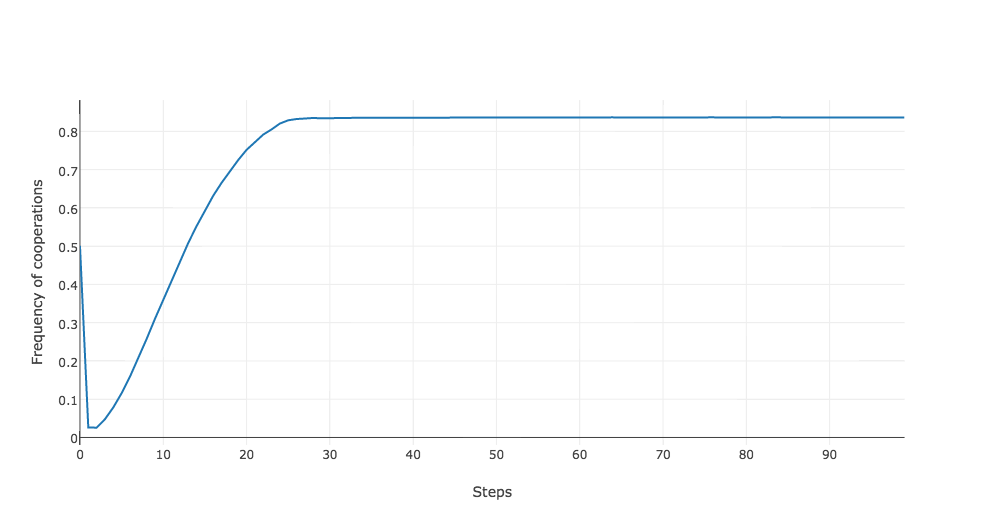
\includegraphics[width=0.8\textwidth]{img/part1/cf-moore-notmyself.png}
\end{figure}

In the plot above, we can see the frequency of cooperation (i.e. the fraction of player cooperating). We can see that starting at $0.5$, it first decrease before stabilizing at around $0.82$.

\subsubsection{Same in every run ?}

\begin{figure}[H]
\centering
   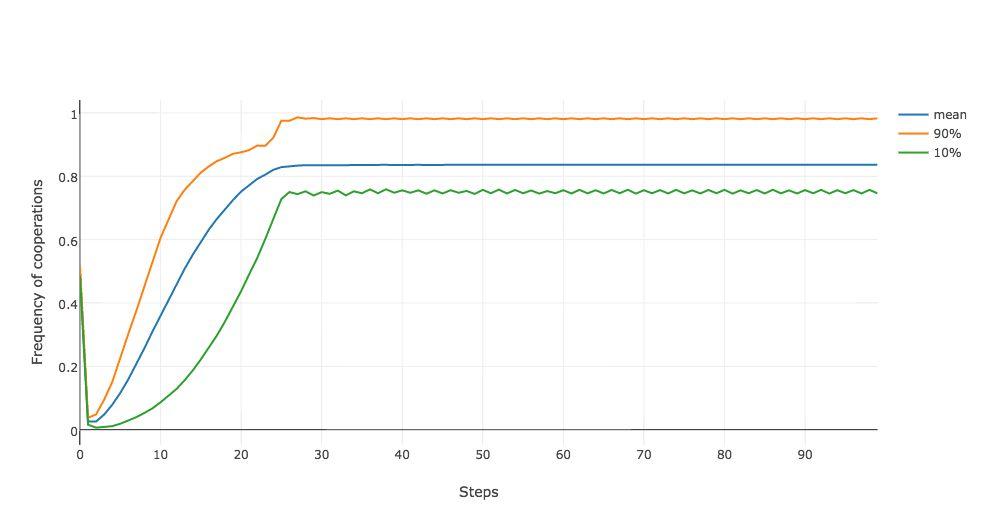
\includegraphics[width=0.8\textwidth]{img/part1/cf-moore-notmyself-90-10.png}
\end{figure}

Answering the question \textit{approximately the same} is quite hard because it's subjective. Above, it is plotted the $0.1$ and $0.9$ quantile. From this plot, one could reasonably say that it is in fact "approximately the same". Note that the $0.1$ and $0.9$ quantile has been chosen because the minimum would be at $0$ and the maximum at $1$.

\subsection{Visualization}

In the visualization below, red is cooperation and blue is defection. We can see some "clusters" getting formatted.

\subsubsection{t=0}

\begin{figure}[H]
\centering
   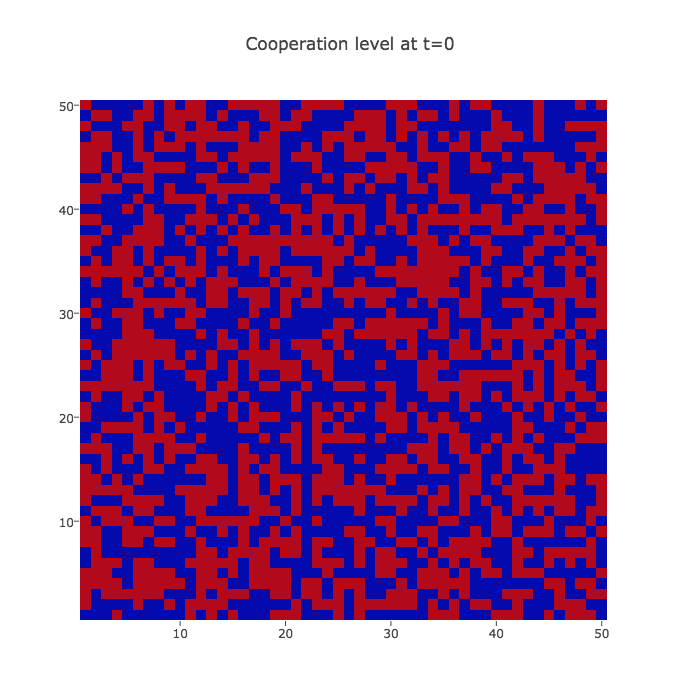
\includegraphics[width=0.6\textwidth]{img/part1/cf-moore-visu-0.png}
\end{figure}

\subsubsection{t=1}

\begin{figure}[H]
\centering
   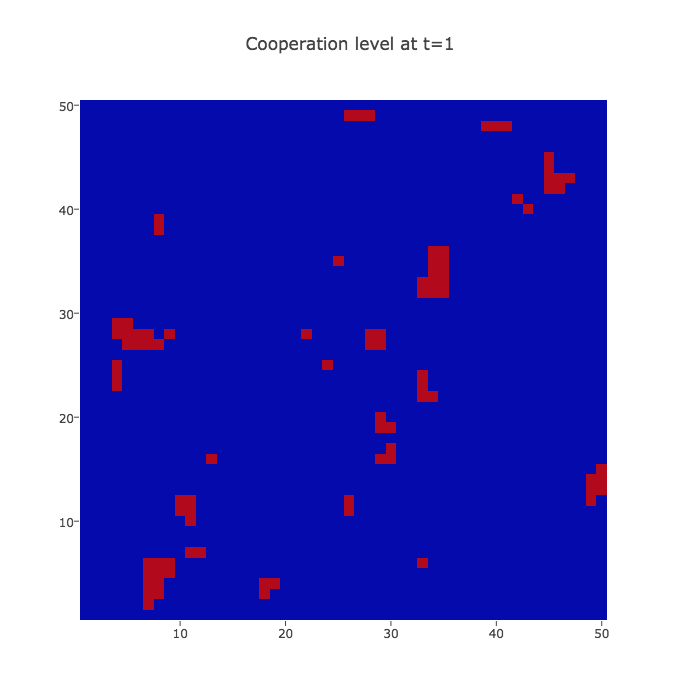
\includegraphics[width=0.6\textwidth]{img/part1/cf-moore-visu-1.png}
\end{figure}

\subsubsection{t=5}

\begin{figure}[H]
\centering
   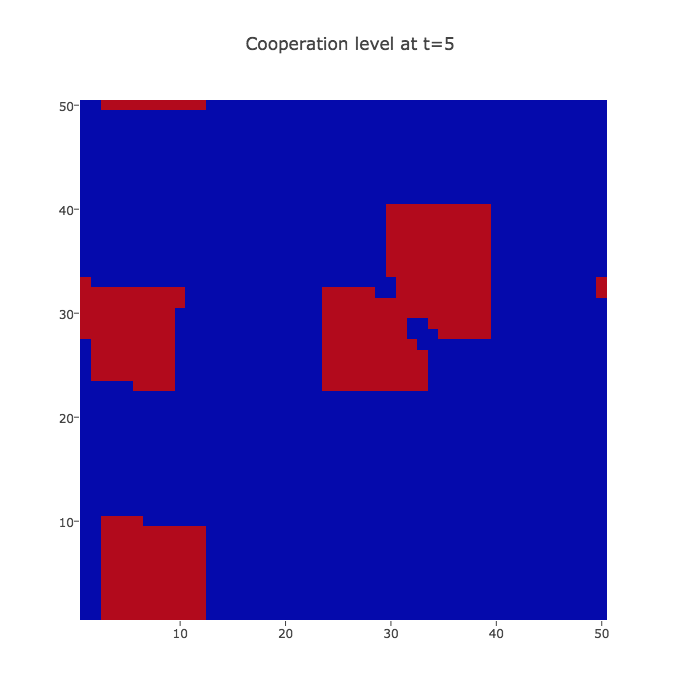
\includegraphics[width=0.6\textwidth]{img/part1/cf-moore-visu-5.png}
\end{figure}

\subsubsection{t=10}

\begin{figure}[H]
\centering
   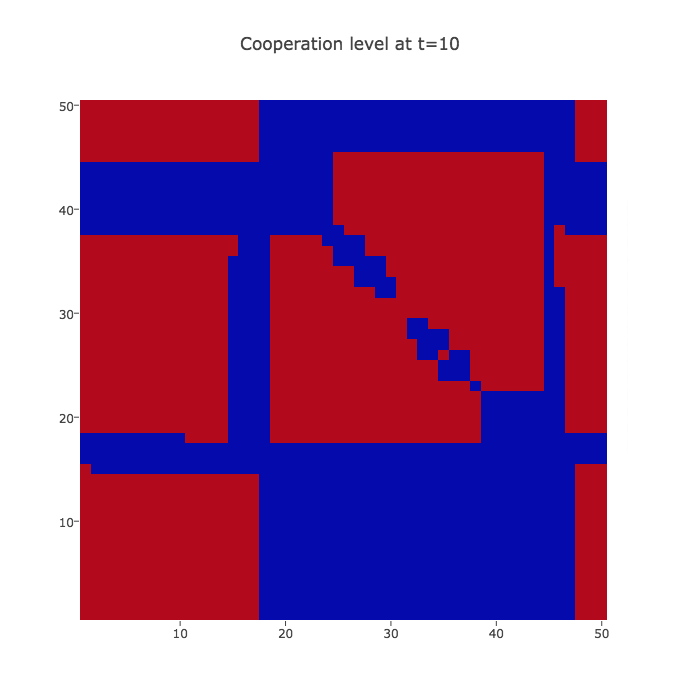
\includegraphics[width=0.6\textwidth]{img/part1/cf-moore-visu-10.png}
\end{figure}

\subsubsection{t=20}

\begin{figure}[H]
\centering
   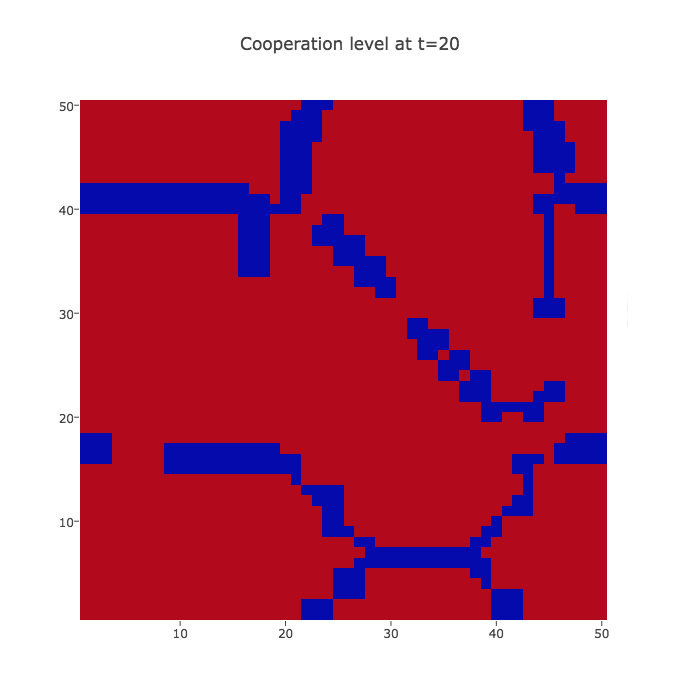
\includegraphics[width=0.6\textwidth]{img/part1/cf-moore-visu-20.png}
\end{figure}

\subsubsection{t=50}

\begin{figure}[H]
\centering
   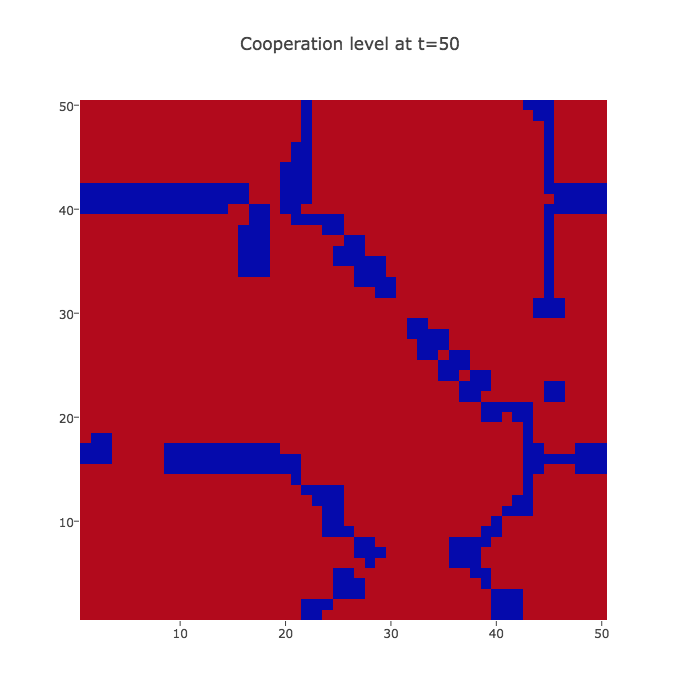
\includegraphics[width=0.7\textwidth]{img/part1/cf-moore-visu-50.png}
\end{figure}

\subsection{Lattice size}

\subsubsection{4x4}

\begin{figure}[H]
\centering
   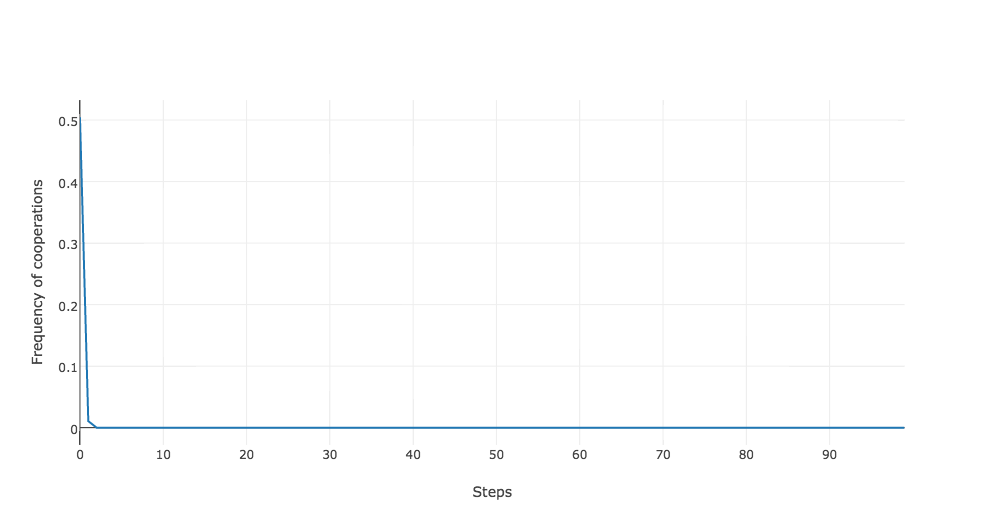
\includegraphics[width=0.6\textwidth]{img/part1/cf-moore-4-4.png}
\end{figure}

\subsubsection{8x8}

\begin{figure}[H]
\centering
   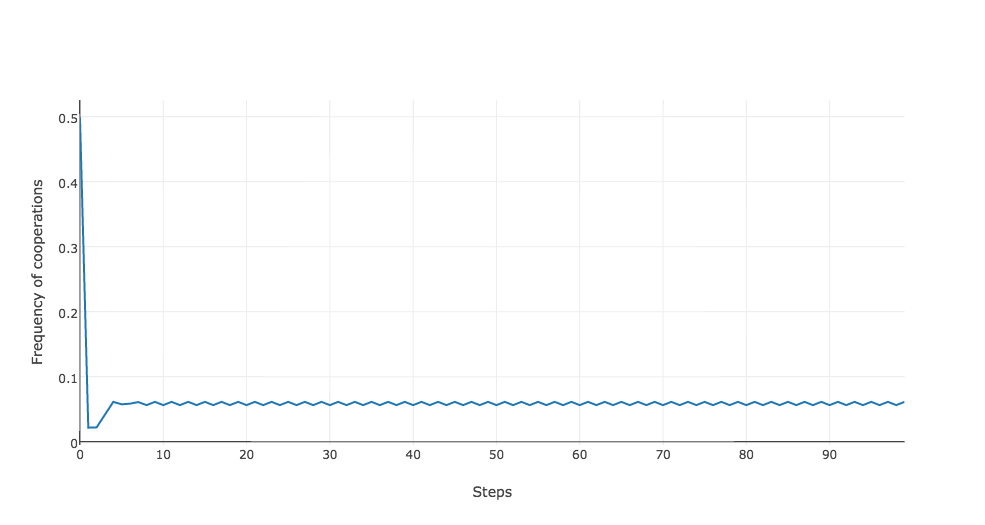
\includegraphics[width=0.6\textwidth]{img/part1/cf-moore-8-8.png}
\end{figure}

\subsubsection{12x12}

\begin{figure}[H]
\centering
   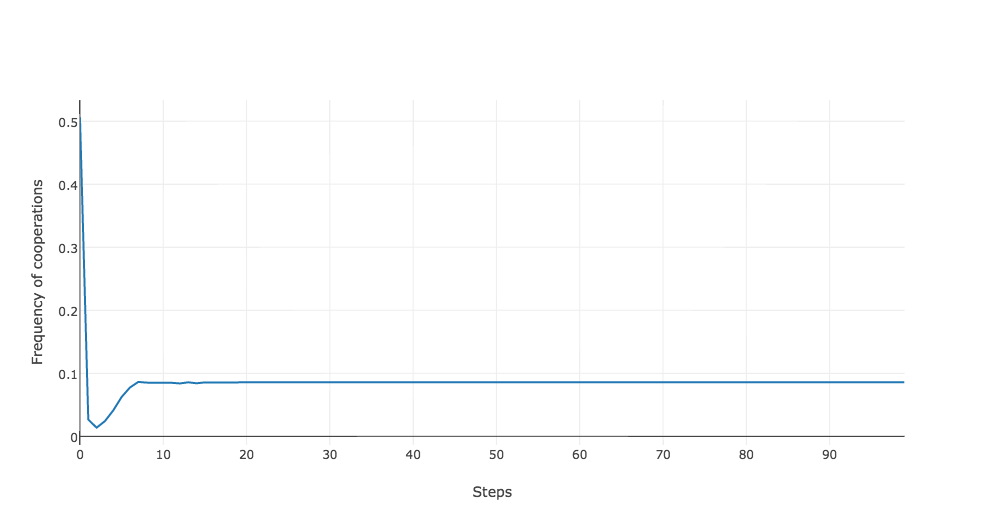
\includegraphics[width=0.6\textwidth]{img/part1/cf-moore-12-12.png}
\end{figure}

\subsubsection{20x20}

\begin{figure}[H]
\centering
   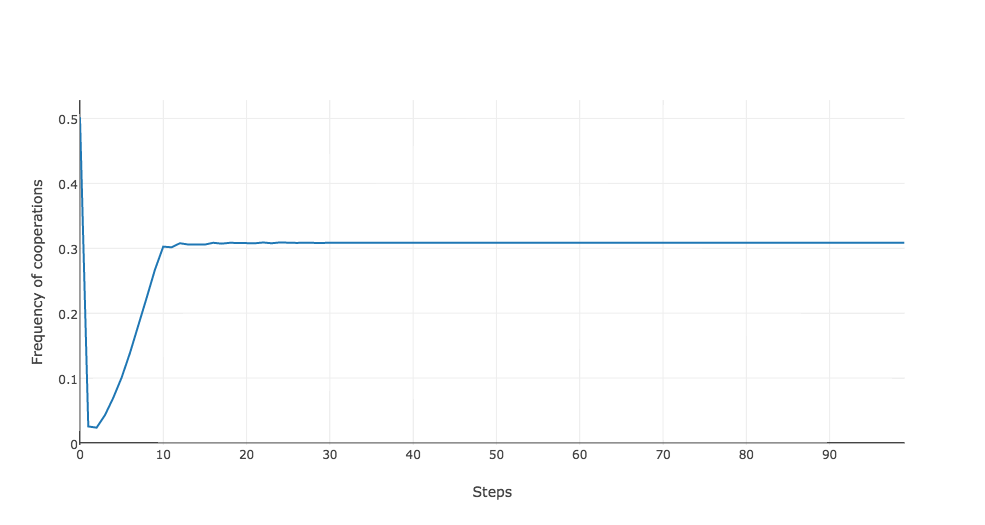
\includegraphics[width=0.6\textwidth]{img/part1/cf-moore-20-20.png}
\end{figure}

\subsubsection{Explanation}

\subsection{Von Neumann}

\subsubsection{Plot}
\begin{figure}[H]
\centering
   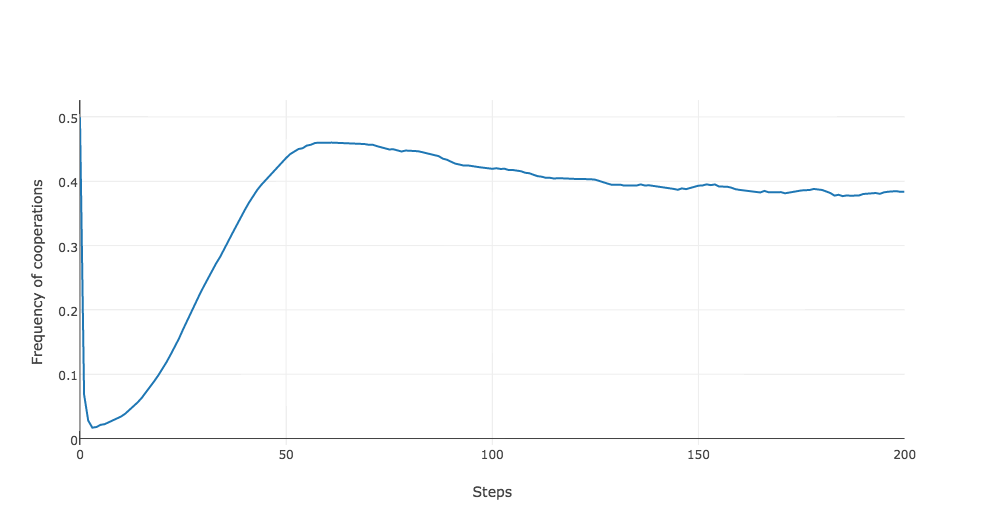
\includegraphics[width=0.8\textwidth]{img/part1/cf-vonn-notmyselfincluded.png}
\end{figure}

\subsubsection{Explanation}
 
\section{Part 2}

\subsection{Probability defined}

$Pij = \frac{1 + [W_j-W_i]/[4*(max\{P,R,T,S\} - min\{P,R,T,S\})]}{2}$ 

This probability makes sense to be defined like that because it indicate the incentive a player has to change is strategy. In other words, the more it can gain by changing his strategy, the more probable he is to change his strategy and will also give him flexibility. 

Indeed, $[W_j-W_i]$ is the payoff difference between the player and his neighbour while $ [4*(max\{P,R,T,S\} - min\{P,R,T,S\})]$ is the maximum possible payoff between the two. The interesting part of the fraction is $[W_j-W_i]/[4*(max\{P,R,T,S\} - min\{P,R,T,S\})]$. It will be equals to 0 if the payoff of the player and his neighbour are equal, negative if the payoff of the player is greater than its neighbour and positive if the payoff of the player is less than its neighbour.

In brief, the probability of switching strategy is closer to 0 if it cost player, $\frac{1}{2}$ if it does not change the outcome for player and close to $1$ if player can win more. It also give player flexibility by allowing him to change to a worse outcome strategy, in order to maybe gain more in the end.

\subsection{Cooperation level}

\subsubsection{Plot}
 
\begin{figure}[H]
\centering
   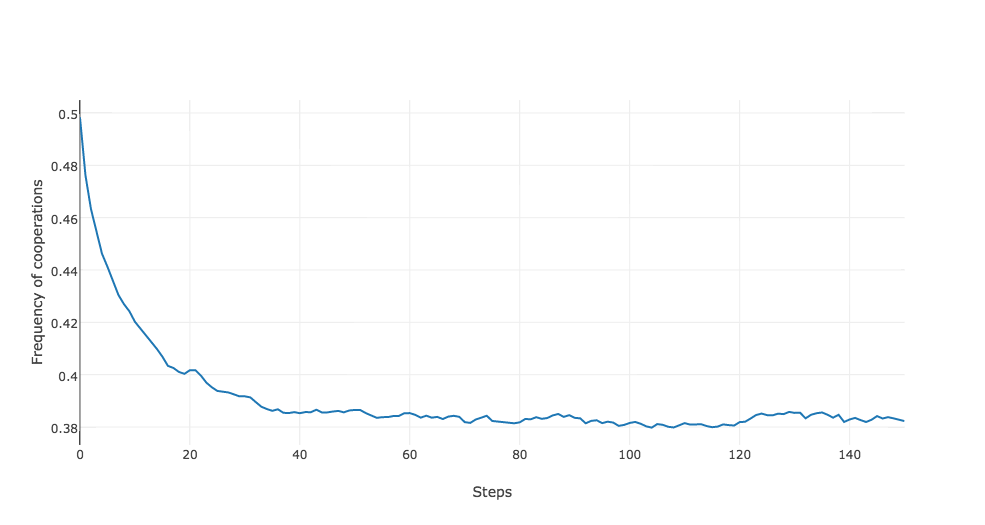
\includegraphics[width=\textwidth]{img/part2/part2-moore-notmyself.png}
\end{figure}

\subsubsection{Same in every run ?}

\begin{figure}[H]
\centering
   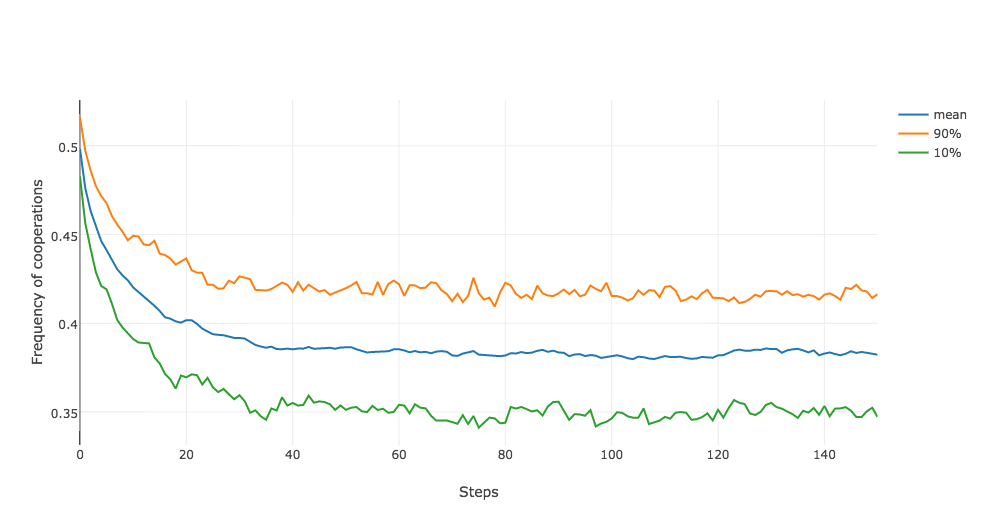
\includegraphics[width=\textwidth]{img/part2/part2-moore-notmyself-std.png}
\end{figure}

\subsection{Visualization}

In the visualization below, red is cooperation and blue is defection. More visualization than asked has been plotted in order to see the stabilisation.

\subsubsection{t=0}

\begin{figure}[H]
\centering
   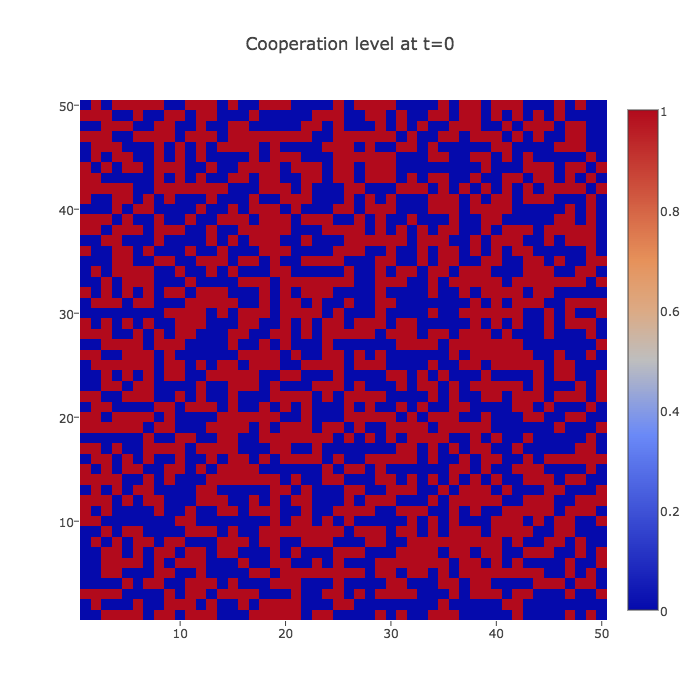
\includegraphics[width=0.6\textwidth]{img/part2/part2-moore-visu-0.png}
\end{figure}

\subsubsection{t=1}

\begin{figure}[H]
\centering
   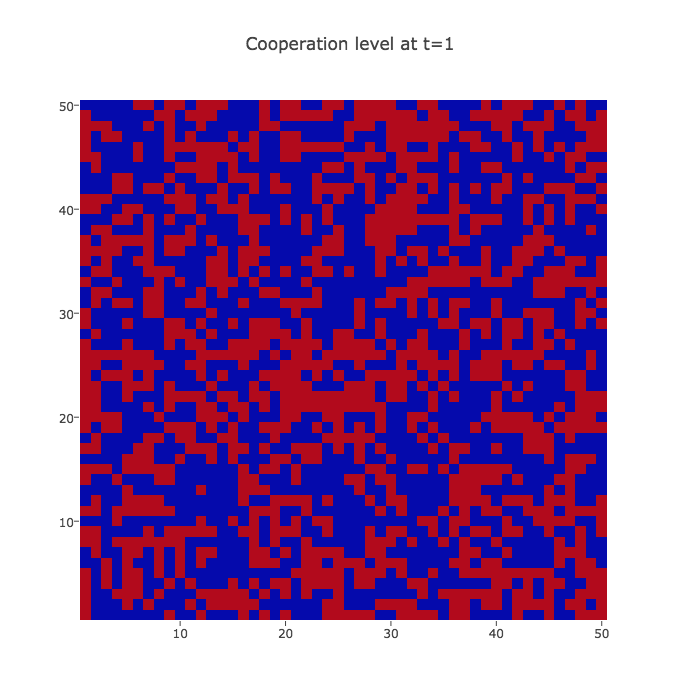
\includegraphics[width=0.6\textwidth]{img/part2/part2-moore-visu-1.png}
\end{figure}

\subsubsection{t=10}

\begin{figure}[H]
\centering
   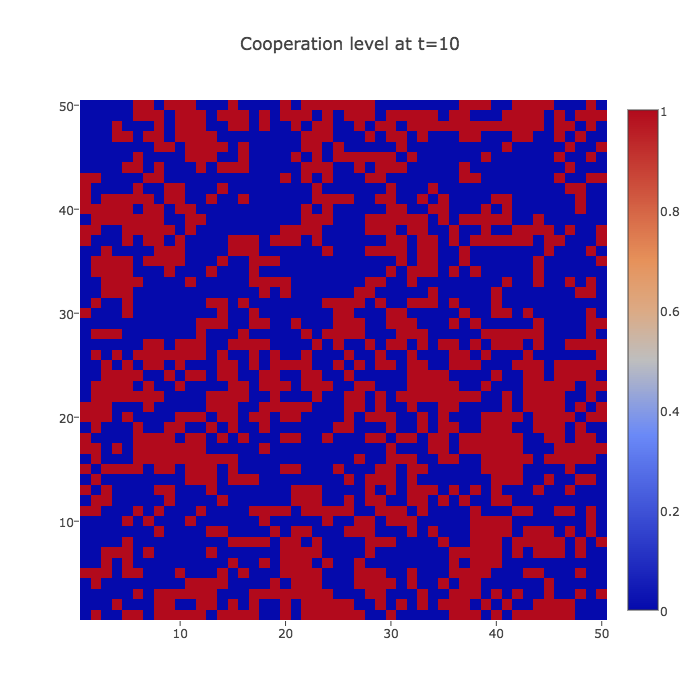
\includegraphics[width=0.6\textwidth]{img/part2/part2-moore-visu-10.png}
\end{figure}

\subsubsection{t=20}

\begin{figure}[H]
\centering
   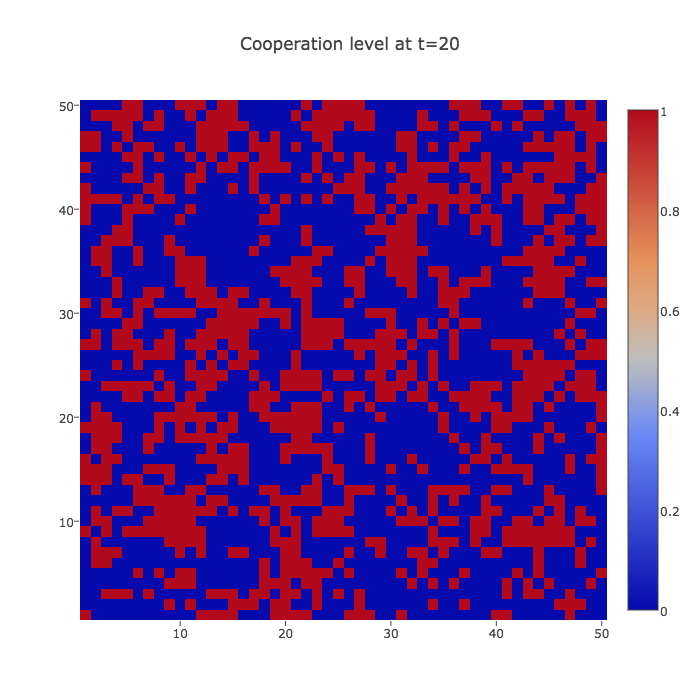
\includegraphics[width=0.6\textwidth]{img/part2/part2-moore-visu-20.png}
\end{figure}

\subsubsection{t=50}

\begin{figure}[H]
\centering
   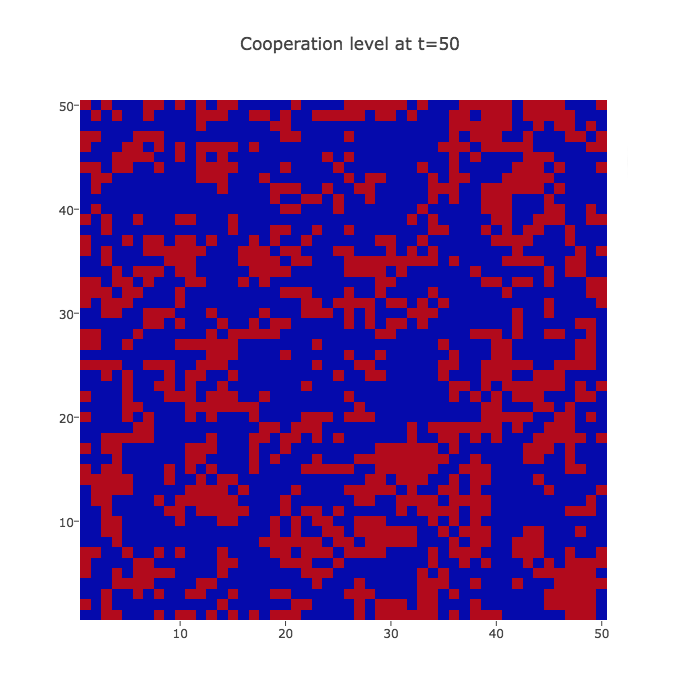
\includegraphics[width=0.6\textwidth]{img/part2/part2-moore-visu-50.png}
\end{figure}

\subsubsection{t=100}

\begin{figure}[H]
\centering
   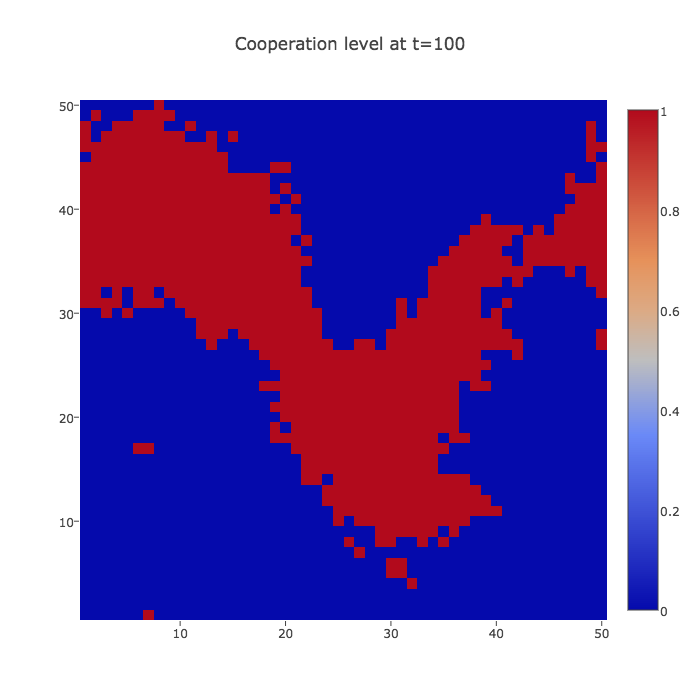
\includegraphics[width=0.6\textwidth]{img/part2/part2-moore-visu-100.png}
\end{figure}

\subsubsection{t=200}

\begin{figure}[H]
\centering
   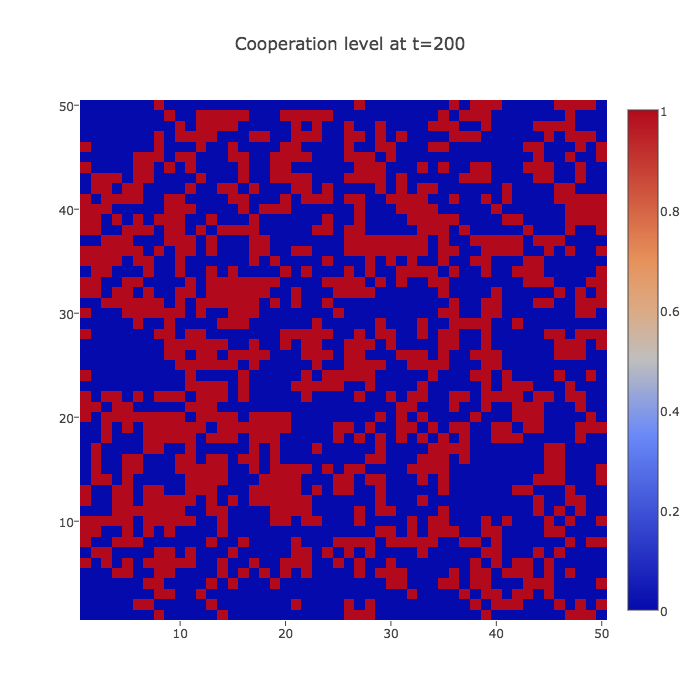
\includegraphics[width=0.6\textwidth]{img/part2/part2-moore-visu-200.png}
\end{figure}

\subsubsection{t=300}

\begin{figure}[H]
\centering
   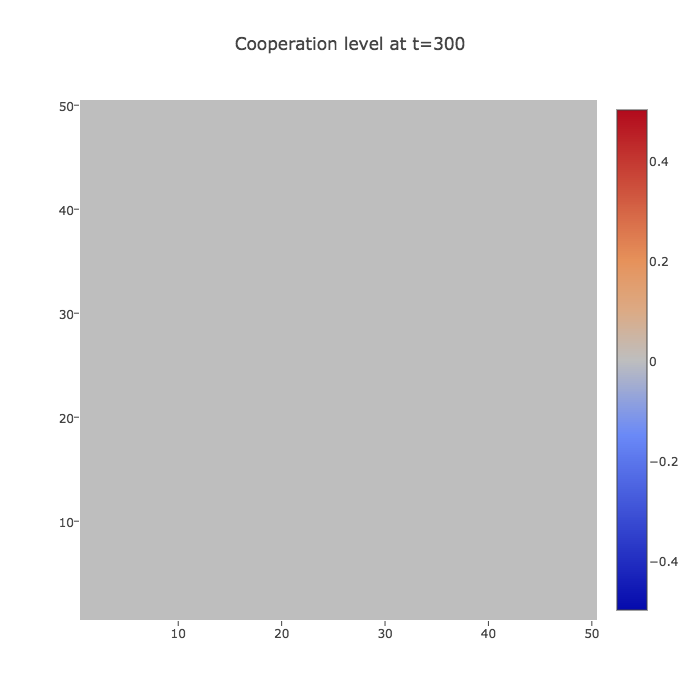
\includegraphics[width=0.6\textwidth]{img/part2/part2-moore-visu-300.png}
\end{figure}

\subsection{Lattice size}

\subsubsection{4x4}

\begin{figure}[H]
   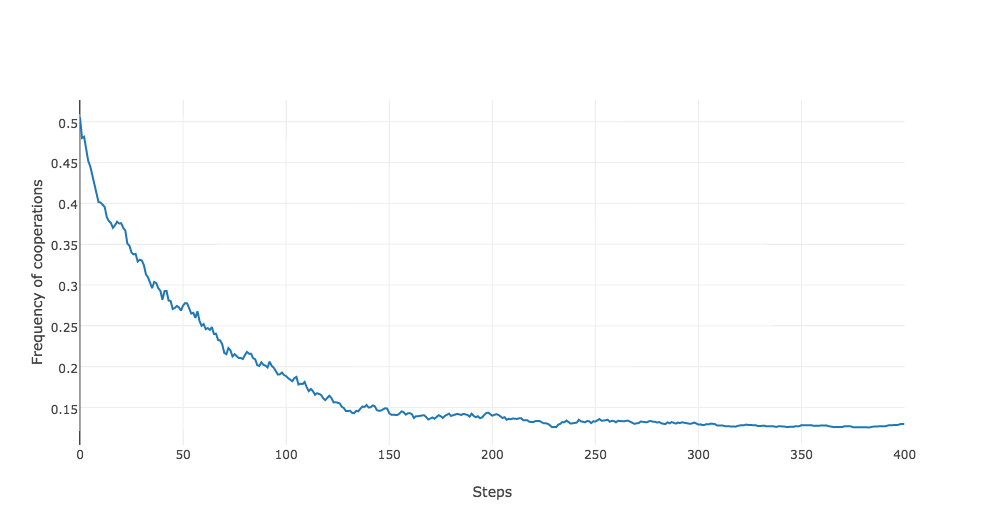
\includegraphics[width=0.7\textwidth]{img/part2/part2-moore-4-4.png}
\end{figure}

\subsubsection{8x8}

\begin{figure}[H]
\centering
   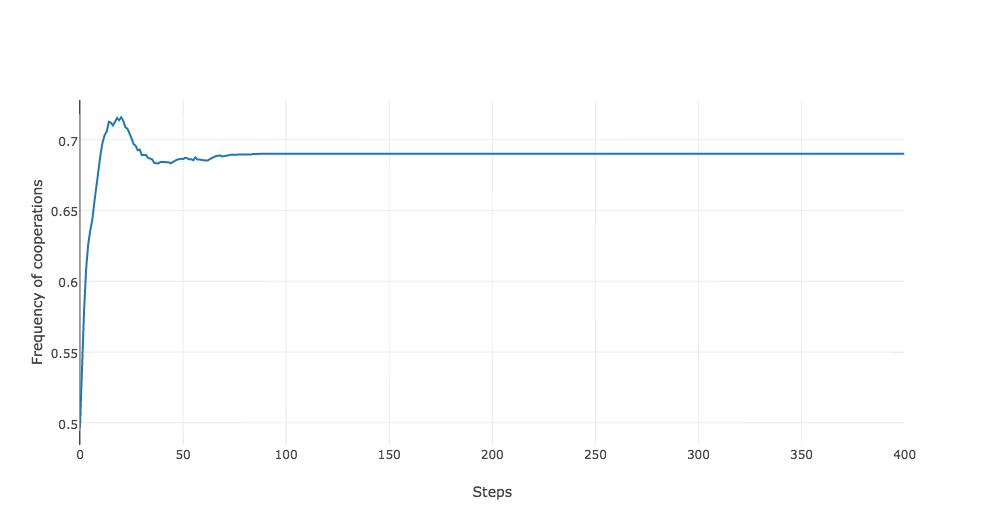
\includegraphics[width=0.7\textwidth]{img/part2/part2-moore-8-8.png}
\end{figure}

\subsubsection{12x12}

\begin{figure}[H]
\centering
   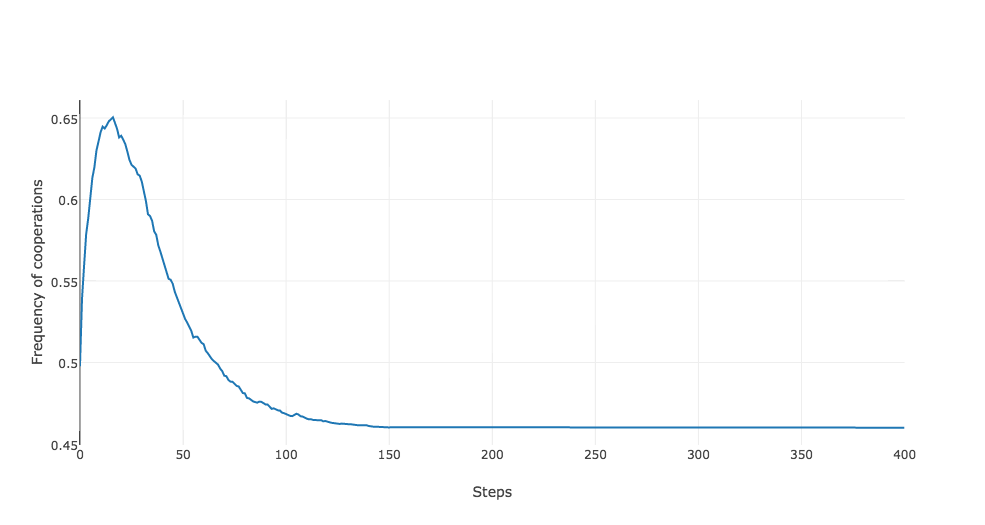
\includegraphics[width=0.7\textwidth]{img/part2/part2-moore-12-12.png}
\end{figure}

\subsubsection{20x20}

\begin{figure}[H]
\centering
   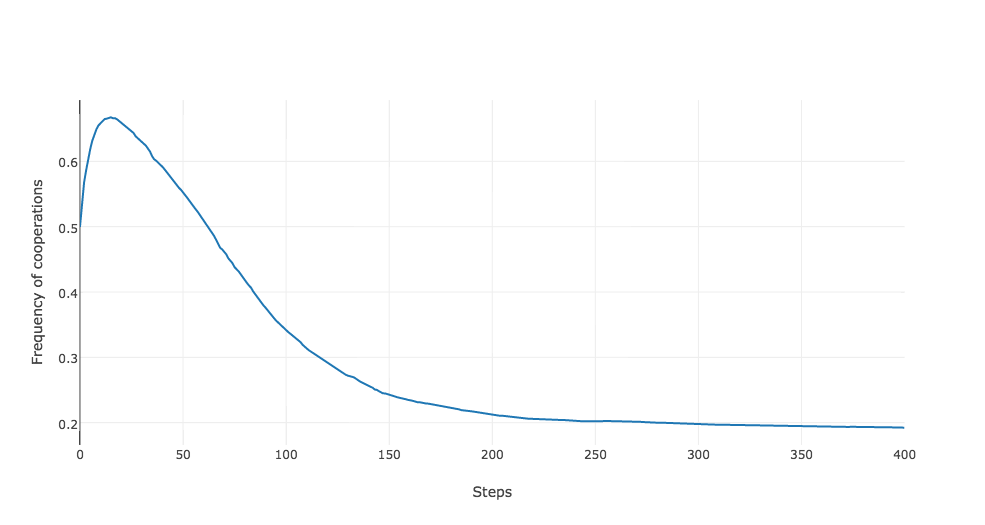
\includegraphics[width=0.7\textwidth]{img/part2/part2-moore-20-20.png}
\end{figure}

\subsubsection{Explanation}


\subsection{Von Neumann}

\begin{figure}[H]
\centering
   \includegraphics[width=0.8\textwidth]{img/part2/part2-vonn-notmyself800.png}
\end{figure}


\section{Part 3 : Bonus}

\end{document}







































              